\section*{Aufgaben 2 und 3}
In dieser Aufgabe sollte die Latenzzeit und die Bandbreite gemessen werden, die
beim kommunizieren zwischen mehreren Prozessen auftreten. Dafür wurde mit verschiedenen
Konfigurationen von beteiligten Prozessoren und Zahlen von Prozessen die Zeit gemessen,
die benötigt wird, um eine Nachricht variabler Länge von einem Prozess zum anderen
und zurück zu senden. Dabei wurde dieser Ablauf $1000$ mal wiederholt und die 
gemessene Zeit gemittelt. Der Quelltext dafür ist in \lref{pingpong} und die darin
aufgerufene Funktion in \lref{walltime} dargestellt.

\lstinputlisting[label=lst:pingpong,caption={pingpong.c}]{../code/02/pingpong.c}
\lstinputlisting[label=lst:walltime,caption={wall\_time.c}]{../code/02/wall_time.c}

Wenn man für alle geforderten Konfigurationen die Zeiten in Abhängigkeit von der
Nachrichtenlänge aufträgt, resultiert der in \fref{zeiten} dargestellte Plot.

\begin{figure}[htb]
  \centering
  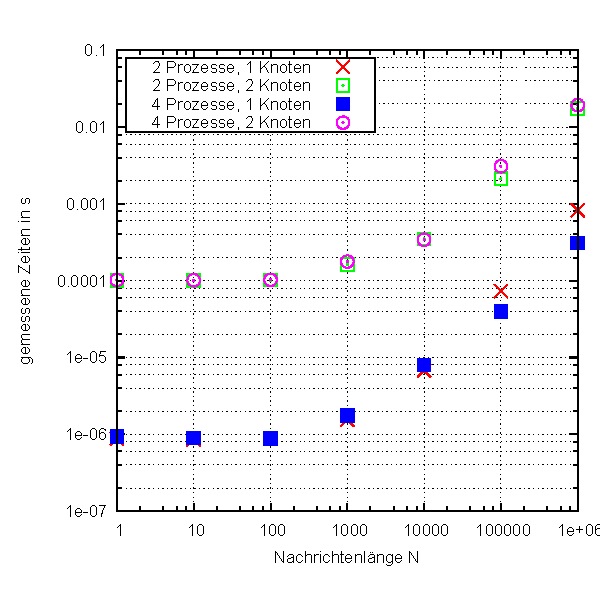
\includegraphics[width=0.8\columnwidth,keepaspectratio]{../tmp/zeiten}
  \caption{Gemessene Zeiten für das Senden einer Nachricht von einem Prozess zum
  anderen und zurück in Sekunden in Abhängigkeit von der Nachrichtenlänge}
  \label{fig:zeiten}
\end{figure}

Wie man erkennen kann, verläuft die Kommunikation zwischen mehreren Knoten generell
langsamer als die zwischen Prozessen, die auf dem gleichen Knoten laufen. Dies war 
zu erwarten, da die einzelnen Knoten über eine vergleichsweise langsame Netzwerkschnittstelle
miteinander verbunden sind, hingegen können die Prozesse auf einem Knoten mit Hilfe
eines internen Busses Informationen austauschen, der deutlich schneller Daten
transportieren kann als externe Verbindungen.

Weiterhin wird deutlich, dass die Nachrichtenlänge für die Arbeit mit mehreren
Knoten für kleine Längen (bis ca. $1000$ Zeichen) kaum einen Einfluss auf die
benötigten Zeiten hat. Demnach ist hier eindeutig die Wahl des Kommunikationsweges
das hemmende Element. Für größere Längen steigt die benötigte Zeit etwa nach einem 
Potenzgesetz (sogar annähernd linear) an. 